\chapter{Kernel Modelling and Identification of Ion Channels}
\label{chap:kernel-modelling}

The previous chapter showed how ion-channel conductances in a conductance-based neuron can be interpreted as memristive elements with fading memory. Throughout this dissertation, we therefore adopt an input-output viewpoint in which these memristive elements are treated as dynamical maps from an input signal to an output signal, and their history dependence is modelled by a \emph{memory functional} that maps past inputs to the present output.

This chapter develops the kernel-based identification framework used in the dissertation for modelling fading-memory memristive elements, instantiated here by ion-channel currents. The technical development, except for the gain-scheduling kernel, is based on a related publication \cite{huo_kernel_modelling_2024}. The presentation is expanded here to fit the dissertation narrative.

\section{Preliminaries}\label{sec:preliminary}
We follow the operator-theoretic viewpoint of \textcite{boyd_fading_1985}. The Euclidean norm on $\R^k$ is denoted by $|\cdot|$. We consider time-invariant, continuous-time, causal systems represented by operators mapping $m$-dimensional input signals to $n$-dimensional output signals.

The input and output spaces of bounded, rate-limited (Lipschitz) signals are denoted by ${\cal U}\subset C^0_b(\R,\R^m)$ and ${\cal Y}\subset C^0_b(\R,\R^n)$, respectively. Input and output trajectories on the entire time axis are denoted by $u_c\in{\cal U}$ and $y_c\in{\cal Y}$. The space of bounded, rate-limited past input signals is denoted by ${\cal U}_\text{past}\subset C^0_b((-\infty,0],\R^m)$.

For $1 \leq p < \infty$, we define $\|u\|_{p}$ for $u:(-\infty, 0]\to\mathbb{R}^m$ by
$$
\|u\|_{p}=\left(\int_{-\infty}^0 |u(t)|^p dt\right)^{1/p},
$$
with analogous definitions on the entire real axis for $u_c\in {\cal U}$:
$$
\|u_c\|_{p}=\left(\int_{-\infty}^{\infty} |u_c(t)|^p dt\right)^{1/p}.
$$
The $L_\infty$ norm is given by
\begin{IEEEeqnarray*}{rCl}
        \norm{u}_\infty &=& \sup_t |u(t)|,
\end{IEEEeqnarray*}
where the supremum is taken over the domain of $u$.

A \emph{system} is an operator $G: {\cal U} \to {\cal Y}$. Let $U_\tau$ denote the delay operator, $(U_\tau u_c)(t):=u_c(t+\tau)$. The system $G$ is said to be \emph{time invariant (TI)} if $GU_\tau u_c=U_\tau Gu_c$. It is \emph{causal} if $u_c(t)=v_c(t)$ for all $t\le0$ implies $(Gu_c)(t)=(Gv_c)(t)$ for all $t\le0$. It is \emph{continuous} if it is a continuous map $G: {\cal U}\to{\cal Y}$.

\textcite{boyd_fading_1985} show that each TI causal operator $G$ has a unique functional $F:{\cal U}_\text{past}\to \R^n$ mapping past input to current output, such that
$$
Fu\coloneqq(Gu)(0).
$$
We call $F$ the \emph{memory functional}. Each TI causal operator $G$ is uniquely determined by its memory functional $F$, and vice versa.

Define $P:{\cal U}\to{\cal U}_\text{past}$ to be the truncation operator, $(Pu_c)(t):=u_c(t)$ for all $t\le 0$. Then
$$
(Gu_c)(t)=FPU_{t}u_c.
$$
Since $PU_{t}$ is a continuous operator, $G$ is continuous if and only if $F$ is continuous \autocite{boyd_fading_1985}. In particular, $F$ is continuous with respect to the uniform norm if: for all $\epsilon>0$, there exists $\delta>0$ such that, for all $u,v\in {\cal U}_\text{past}$,
$$
\sup_{t\le0}|u(t)-v(t)|<\delta \Rightarrow  |Fu-Fv|<\epsilon.
$$

Let $H$ be a map between arbitrary normed spaces $\cal U$ and $\cal Y$. If, for all $u,v \in \cal U$,
\begin{IEEEeqnarray*}{rCl}
        \norm{Hu - Hv}_{\cal Y} \leq \lambda \norm{u - v}_{\cal U},
\end{IEEEeqnarray*}
then $\lambda$ is said to be a \emph{Lipschitz constant} of $H$, and $H$ is said to be Lipschitz. This definition applies equally to operators and memory functionals.

An operator $H$ is described as having \emph{incremental small gain} if its Lipschitz constant is at most $1$ when both normed spaces are equipped with the $L_2$ norm. This constant provides an input-output bound on incremental gain and is a useful robustness metric for interconnections.

\section{Kernel Modelling of Fading Memory Systems}\label{chap:kernel}

\subsection{Fading memory}
Fading memory is a regularity property that expresses that the influence of older inputs on the current output decays as they recede into the past. In their seminal work, \textcite{boyd_fading_1985} introduced fading memory in system approximation and showed that Volterra series are universal approximators of fading-memory operators. The concept also plays a role in robust control \autocite{shamma_fading-memory_1993,Sandberg1994}. More recently, \textcite{Gonon2022} introduced the \emph{reservoir kernel} as a universal approximant for the Volterra expansion of a fading-memory operator.

We use the weighted-norm viewpoint of \textcite{matthews_identification_1994} and the fading-memory normed spaces of \textcite{grigoryeva_echo_2018}. For $p=2$, this gives the past-input space a Hilbert-space structure and enables a direct kernel representation of the memory functional.

Let $w: (-\infty, 0] \to (0, 1]$ be a weight such that $\lim_{t\to-\infty}w(t)=0$ and $w$ has finite $L_p$ norm for all $ 1 \leq p\leq \infty$. We define the $(w, p)$ fading memory norm of a past signal $u$ as
$$
\|u\|_{w,p}:=\|u\,w\|_{p},
$$
and the corresponding $(w,p)$ fading-memory normed space as
$$
{\cal W}_{w, p} \coloneqq \{u:(-\infty, 0] \to \R^{m} \mid \|u\|_{w, p}< \infty\}.
$$
Note that ${\cal U}_\text{past}\subset {\cal W}_{w, p}$.

In this chapter, except Section~\ref{sec:incremental small gain_pass}, we restrict attention to the case $p=2$ and denote the norm by $\|u\|_{{\cal U}_\text{past}}:=\|u\|_{w, 2}$. In this case, we also have an inner product, denoted by
$$
\left\langle u,v \right\rangle_{{\cal U}_\text{past}}=\left\langle u,v \right\rangle_{w}:=\langle uw,vw\rangle,
$$
where $\langle u,v \rangle$ is the standard $L_2$ inner product. Fading memory is then defined as continuity with respect to a fading-memory norm.

\begin{definition}\label{fading memory definition}
Consider an operator $G: {\cal U} \to {\cal Y}$. We say that $G$ has $(w, p)$ \emph{fading memory} if and only if its memory functional $F:{\cal U}_\text{past}\to \R^{n}$ is continuous with respect to the $(w,p)$ fading memory norm: for all $ \epsilon>0$, there exists $\delta>0 $ such that, for all $u, v \in {\cal U}_\text{past}$,
\begin{IEEEeqnarray*}{+rCl+x*}
\|u-v\|_{w, p}<\delta &\Rightarrow&  |Fu-Fv|< \epsilon.
&\qedhere
\end{IEEEeqnarray*}
\end{definition}

\subsection{Problem Statement}
We address the problem of learning the fading-memory functional $F$ of a system from input-output data.
\begin{objective}
Given $\{(u_{c,i},y_{c,i})\in {\cal U} \times {\cal Y} \}_{i=1}^l$ and a finite set of sampling times $\mathcal{T}$, find $\hat{F}$ that satisfies Definition~\ref{fading memory definition} and minimizes
$$
\sum_{t\in\mathcal{T}}\sum_{i=1}^{l}\left|\hat{F}PU_{t}u_{c,i}-y_{c,i}(t)\right|^2.
$$
\end{objective}
Let $u_{i,t}=PU_{t}u_{c,i}\in{\cal U}_\text{past}$ and $y_{i,t}=y_{c,i}(t)\in\R^n$. Re-indexing the data as a single set of pairs $\{(u_j,y_j)\}_{j=1}^{M}$ with $M=l\,\text{card}(\mathcal{T})$, we obtain the equivalent regression problem:
\begin{objective}
Given $\{(u_{j},y_{j})\in {\cal U}_{\text{past}} \times \R^n \}_{j=1}^{M}$, find $\hat{F}$ that satisfies Definition~\ref{fading memory definition} and minimizes
$$
\sum_{j=1}^{M}\left|\hat{F}u_{j}-y_{j}\right|^2.
$$
\end{objective}
Beyond data fit, we are particularly interested in enforcing incremental input-output properties such as incremental small gain. Section~\ref{sec:incremental small gain_pass} discusses the extension to other properties.

\subsection{Kernel Representation of Fading Memory Functionals}\label{sec:kernel_approx}
Approximation theory in reproducing kernel Hilbert spaces (RKHSs) is classical for continuous functions in finite-dimensional spaces \autocite{paulsen_introduction_2016} and has been extended to arbitrary separable Hilbert spaces \autocite{christmann_universal_2010}. We combine these results with vector-valued kernels \autocite{micchelli_learning_2005} to approximate continuous vector-valued functionals on compact subsets of ${\cal U}_\text{past}$. Let ${\cal H}$ denote an RKHS of functionals $F:{\cal U}_\text{past}\to\R^n$ with inner product $\langle\cdot,\cdot\rangle_{\cal H}$.

\begin{definition}[RKHS]
A mapping $k:{\cal U}_\text{past} \times {\cal U}_\text{past} \to {\cal B}(\R^n)$, where ${\cal B}(\R^n)$ denotes bounded linear operators on $\R^n$, is called a \textit{reproducing kernel} of ${\cal H}$ if:
\begin{enumerate}
    \item $k(\cdot,u)\alpha:{\cal U}_\text{past}\to\R^n$ is a member of ${\cal H}$ for all $u\in {\cal U}_\text{past}$ and $\alpha \in \R^n$.
    \item The \textit{reproducing property} holds: for all $u\in{\cal U}_\text{past}$, $\alpha \in \R^n$, and $F\in {\cal H}$,
    $$\langle \alpha,Fu\rangle=\langle F,k(\cdot,u)\alpha\rangle_{{\cal H}} \qedhere$$
\end{enumerate}
\end{definition}

\begin{definition}[Universal kernel \cite{caponnetto_universal_2008}]
Let $C^0(S,\R^{n})$ be the set of all continuous functionals mapping a compact set $S\subset{\cal U}_\text{past}$ to $\R^n$. If ${\cal H}$ is dense in $C^0(S,\R^{n})$, then the corresponding kernel $k$ is called a \emph{universal kernel} on $C^0(S,\R^{n})$.
\end{definition}

The following theorem of \textcite{christmann_universal_2010} shows how to construct universal kernels on compact subsets of separable Hilbert spaces.
\begin{theorem}[\text{\autocite[Thm. 2.2]{christmann_universal_2010}}]
Let $S$ be a compact subset of a separable Hilbert space with inner product $\langle\cdot,\cdot\rangle_{{\cal U}_\text{past}}$. Let $\sigma(\cdot):\R\to\R$ be a function that can be expressed by its Taylor series
$$
\sigma(t)=\sum_{n=0}^{\infty}c_nt^n.
$$
If $c_n>0$ for all $n$ then the kernel $k:{\cal U}_\text{past}\times {\cal U}_\text{past}\to \R$,
$$
k(u,v)=\sigma(\langle u,v\rangle_{{\cal U}_\text{past}}),
$$
is a universal kernel of $C^0(S,\R)$.
\end{theorem}

Any universal kernel in $C^0(S,\R)$ induces a corresponding universal kernel in $C^0(S,\R^n)$:
\begin{theorem}
For any universal kernel $k$ in $C^0(S,\R)$, the kernel
$$
k_e(u,v)=k(u,v)I
$$
is universal in $C^0(S,\R^n)$, where $I$ is the $n\times n$ identity matrix.
\end{theorem}

\begin{proof}
Let \(F\in C^0(S,\R^n)\) with components \(F=(F_1,\dots,F_n)^\top\). For each \(j\in\{1,\dots,n\}\) and any \(\epsilon>0\), universality of \(k\) implies that there exist an integer \(l_j\), centers \(A_j:=\{u_{j,i}\}_{i=1}^{l_j}\subset S\), and coefficients \(\{\alpha_{j,i}\}_{i=1}^{l_j}\subset\R\) such that
\[
\sup_{u\in S} \left|F_j(u)-\sum_{i=1}^{l_j}\alpha_{j,i}\, k(u_{j,i},u)\right| < \frac{\epsilon}{\sqrt{n}}.
\]
Define $\alpha_{j}(u_i)=\alpha_{j,i}$ for all $u_i \in A_j$ and let
\[
A:=\bigcup_{j=1}^n A_j,
\]
and enumerate \(\{u_{m}\}_{m=1}^{M}:=A\), where $M=\text{Card}(A)$. For each \(j\), define
\[
\hat{F}_j(u)=\sum_{m=1}^{M}\tilde{\alpha}_{j}(u_m)\, k(u_{m},u),
\]
where \(\tilde{\alpha}_{j}(u_m)=\alpha_{j}(u_m)\) if \(u_{m}\in A_j\) and zero otherwise. Let \(\hat{F}(u):=(\hat{F}_1(u),\dots,\hat{F}_n(u))^\top\). Then
\[
|F(u)-\hat{F}(u)|_2 \le \sqrt{n}\max_{1\le j\le n}\sup_{u\in S}|F_j(u)-\hat{F}_j(u)| < \epsilon.
\]
Since \(\hat{F}\) is a finite linear combination of the kernel sections \(k_e(u_m,\cdot)=k(u_m,\cdot)I\), it belongs to the RKHS of \(k_e\). As \(\epsilon>0\) was arbitrary, the RKHS of \(k_e\) is dense in \(C^0(S,\R^n)\).
\end{proof}

A particular example of a universal kernel on $C^0(S,\R^n)$ is the Gaussian-type radial basis function (RBF) kernel with $\sigma\neq0$:
$$
k_e(u,v)=I\operatorname{exp}\left(-\frac{\|u-v\|_{{\cal U}_\text{past}}^2}{2\sigma^2}\right).
$$

If $S$ is compact in ${\cal U}_\text{past}$, universal kernels allow approximation of any $F\in C^0(S,\R^n)$. A standard compact set (already used by Boyd and Chua) is the set of bounded, rate-limited past inputs
$$
S_b:=\left\{u\in {\cal U}_\text{past}\,\middle|\,|u(t_1)-u(t_2)|\le C_1|t_1-t_2|,\ \sup_{t\le 0} |u(t)|\le C_2\right\},
$$
for some $0<C_1,C_2<\infty$ and all $t_1,t_2\leq 0$.

\subsection{Kernel-Regularized Learning of Memory Functionals}
Kernel methods are popular in machine learning for their ability to regularize the data fit of the approximation. Given a finite data set of past inputs and current outputs, together with a fading-memory kernel, the representer theorem provides an optimal approximant within the RKHS.

\begin{theorem}[Representer Theorem \protect{\autocite[Thm. 8.7]{paulsen_introduction_2016}}]
Given $l$ past inputs and current outputs $(u_i,y_i) \in S_b \times \R^n$, let $\hil$ be an RKHS of functionals from $S_b$ to $\R^n$. Then the regularized least-square problem
$$
\min_{\hat F \in {\cal H}} \sum_{i=1}^{l}\left|\hat{F}u_{i}-y_i\right|^2+\gamma\|\hat{F}\|^2_{\hil}
$$
has a unique solution of the form
$$
\hat{F}u=\sum_{i=1}^{l}\alpha_ik(u_{i},u),\quad \hat{\alpha}=(K+\gamma I)^{-1}Y,
$$
where $\hat{\alpha}$ is a matrix whose $i$th row is $\alpha_i^\top$, $K_{i,j}=k(u_{i},u_{j})$, and $Y$ is the matrix whose $i$th row is $y_i^\top$.
\end{theorem}

The regularized least-squares problem combines an empirical loss and the RKHS norm of the functional. The parameter $\gamma$ controls the trade-off between data fit and regularization, and typically improves robustness to noise and generalization.

Regularization also provides a convenient way to enforce incremental small gain. We next relate the Lipschitz constant of the memory functional (with respect to a fading-memory norm) to an incremental $L_2$ gain bound for the induced operator.

First, we define \emph{Lipschitz kernels}.
\begin{definition}
A kernel $k(u,v)$ is said to have \emph{Lipschitz constant $r$} if
\begin{equation}
|k(u,u)-2k(u,v)+k(v,v)|\le r^2\|u-v\|_{{\cal U}_\text{past}}^2, \label{eq:continuous_kernel}
\end{equation}
for some $r>0$. It is called a \emph{nonexpansive kernel} in \autocite{van_waarde_kernel-based_2023} when $0< r\le1$.
\end{definition}
If a kernel has Lipschitz constant $r$, then
$$
|\hat{F}u-\hat{F}v|\le r\|\hat{F}\|_{\hil }\|u-v\|_{{\cal U}_\text{past}}.
$$
This is a direct application of \autocite{van_waarde_kernel-based_2023}[Lemma 1]. Van Waarde and Sepulchre \autocite{van_waarde_kernel-based_2023}[Prop.~2] provide several examples of kernels which satisfy~\eqref{eq:continuous_kernel}. In particular, the Gaussian-type RBF kernel is universal with Lipschitz constant $r=\frac{1}{\sigma^2}$. We now give a condition on the Lipschitz constant of the functional which guarantees incremental small gain of the induced operator.

\begin{theorem}[Incremental small gain regularization]\label{cor:regularization}
Let ${\cal U}_\text{past}$ be equipped with the norm $\left\|\cdot\right\|_{{\cal U}_\text{past}}^2=\left\|\cdot\right\|_{w,2}^2$. Assume that the weight function $w$ satisfies
$$
c \coloneqq \left(\int_{-\infty}^{0}w(t)^2dt\right)^{\frac{1}{2}}<\infty.
$$
Suppose $G: {\cal U} \to {\cal Y}$ and its memory functional $F:{\cal U}_\text{past}\to \R^n$ is Lipschitz with respect to $\left\|\cdot\right\|_{{\cal U}_\text{past}}$ with constant $\beta$. Then $G$ has incremental small gain if $\beta^2<\frac{1}{c^2}$.
\end{theorem}

\begin{proof}
For $u_c,v_c\in\{u_c\in {\cal U} \mid \left\|u_c\right\|_2<\infty\}$, let $u(t,\cdot)$ and $v(t,\cdot)$ denote the truncated $u_c$ and $v_c$ at time $t$, defined by
$$
u(t,\tau)=
\begin{cases}
    u_c(t+\tau) & \tau\le 0, \\
    0 & \tau>0.
\end{cases}
$$
It follows that $Pu(t,\cdot), Pv(t,\cdot)\in {\cal U}_\text{past}$. We then have
\begin{IEEEeqnarray*}{rCl}
\|Gu_c-Gv_c\|_2^2&=&\int_{-\infty}^{\infty}|Gu_c(t)-Gv_c(t)|^2 dt\\
&=&\int_{-\infty}^{\infty}|FPu(t,\cdot)-FPv(t,\cdot)|^2 dt\\
&\leq&\int_{-\infty}^{\infty}\beta^2\|Pu(t,\cdot)-Pv(t,\cdot)\|_{{\cal U}_\text{past}}^2 dt.
\end{IEEEeqnarray*}
\vspace{-20pt}
$$
=\int_{-\infty}^{\infty}\beta^2 \int_{-\infty}^{0}|u_{c}(t+\tau)-v_{c}(t+\tau)|^2w(\tau)^2d\tau dt.
$$
Let $w'(\tau)=w(\tau)$ for $\tau\le0$ and $w'(\tau)=0$ for $\tau>0$. Then
$$
\|Gu_c-Gv_c\|_2^2=\int_{-\infty}^{\infty}\beta^2 \int_{-\infty}^{\infty}|u_c(\tau)-v_c(\tau)|^2w'(t+\tau)^2d\tau dt.
$$
Since $w'$ is square integrable, Fubini's theorem yields
$$
\|Gu_c-Gv_c\|_2^2=\int_{-\infty}^{\infty}\beta^2 |u_c(\tau)-v_c(\tau)|^2\left(\int_{-\infty}^{\infty}w'(t+\tau)^2dt\right) d\tau.
$$
Note that $\int_{-\infty}^{\infty}w'(t+\tau)^2dt=c^2$, so
$$
\|Gu_c-Gv_c\|_2^2=c^2 \int_{-\infty}^{\infty}\beta^2 |u_c(\tau)-v_c(\tau)|^2d\tau
=\beta^2c^2\|u_c-v_c\|_2^2.
$$
If $\beta^2<\frac{1}{c^2} $, it follows that the operator $G$ has incremental small gain.
\end{proof}

To impose incremental small gain on the approximated system, as described in Theorem~\ref{cor:regularization}, it suffices to choose a sufficiently large value for $\gamma$. There is an expected trade-off: enforcing a smaller gain typically requires stronger regularization and may increase bias. We can also use this small-gain mechanism to impose other IQC properties via a scattering transform \autocite{van_waarde_kernel-based_2023}.

\subsection{Regularized Learning with IQC Constraints}\label{sec:incremental small gain_pass}
A system $G$ is said to be \emph{incrementally passive} if its input space ${\cal X}$ and output space ${\cal Y}$ are the same Hilbert space and $\langle Gx_1-Gx_2, x_1-x_2\rangle \geq 0$ for all $x_1,x_2\in {\cal X}$.
\begin{theorem}[Scattering transform between incremental small gain and incremental passivity]
If a system $E$ has incremental small gain and its input and output spaces coincide, then $G:=(I-E)(I+E)^{-1}$ is incrementally passive. Conversely, if a system $G$ is incrementally passive, then $E:=(I-G)(I+G)^{-1}$ has incremental small gain.
\end{theorem}
As in \autocite{van_waarde_kernel-based_2023}, a small-gain constraint can be converted to other IQCs through a scattering transform. We use incremental passivity as the example. In the present neuromorphic setting, individual ionic currents are interpreted as memristive conductance elements: they have memory through internal state, but at each instant they still act as input-output elements in a circuit interconnection. Imposing incremental passivity therefore biases the learned current toward dissipative interconnection behaviour, consistent with operator-theoretic viewpoints based on monotonicity and incremental dissipativity \cite{sepulchre_spiking_2022,sepulchre_incremental_2022}. The transform admits an implementation through a feedback circuit \autocite{anderson_small-gain_1972}, depicted in Figure~\ref{fig:scattering}.
\begin{figure}[H]
    \centering
    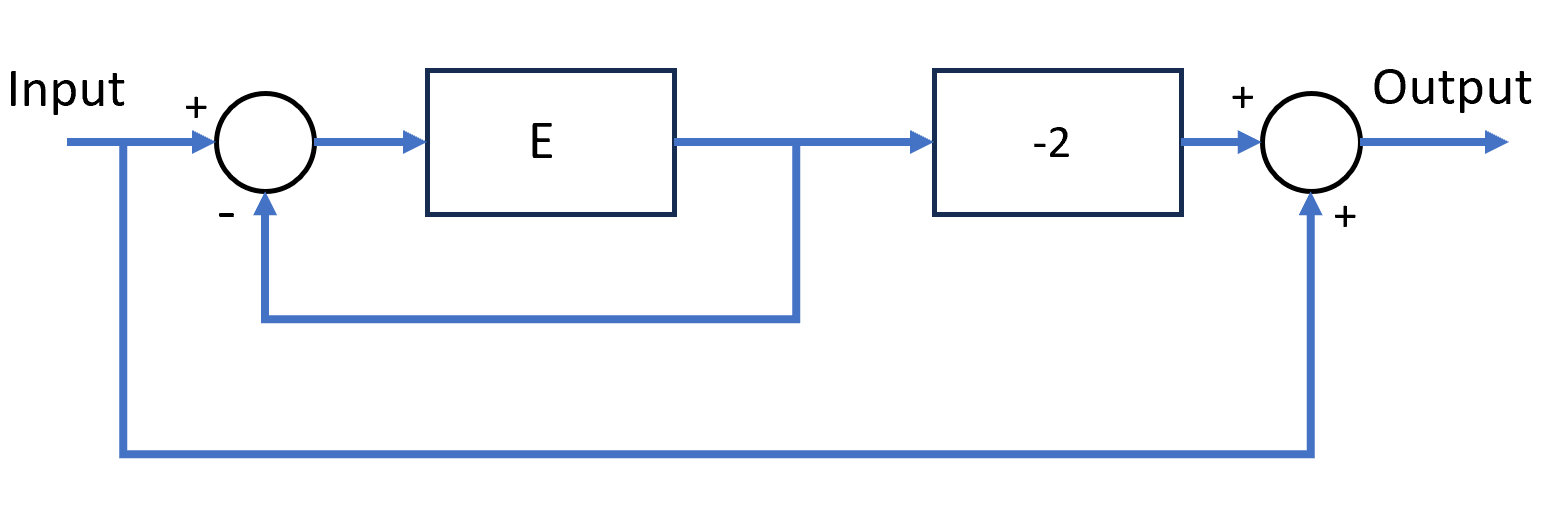
\includegraphics[scale=0.6]{figures/03_Kernel_Modelling_and_Identification_of_Neuromorphic_Elements/codes/scattering.png}
    \caption{Block diagram implementation of scattering transform in \cite[fig 4(a)]{anderson_small-gain_1972}. $E$ is an incremental small gain system and the overall system is an incrementally passive system.}\label{fig:scattering}
\end{figure}

To impose incremental passivity, we use the scattering transform to convert input/output data of system $G$ into input/output data of the incremental small gain system $E$. Let $\{u_i(\cdot),y_i(\cdot)\}_{i=1}^{N}$ represent $N$ truncated past input/output signals from $G$, with $u_i,y_i\in{\cal U}_\text{past}$. Applying the transform yields new pairs $\{u_i',y_i'\}_{i=1}^{N}$, where $u_i'=\frac{1}{2}(u_i+y_i)$ and $y_i'=\frac{1}{2}(u_i-y_i)$. We then learn the memory functional that maps $u_i'$ to $y_i'(0)$ using a sufficiently large $\gamma$ to ensure small gain. Finally, connecting $E$ as depicted in Figure~\ref{fig:scattering} yields an incrementally passive approximation of $G$.

For a strictly proper LTI system $G$, the transformed system $E$ might not be strictly proper. Hence $E$ may fail to be continuous with respect to the pure $L_2$ fading memory norm. To accommodate an instantaneous (time-$0$) component, we equip ${\cal U}_\text{past}$ with the modified norm
$$
\|x\|:=\left(a\|x\|_{w,2}^2 + b|x(0)|^2\right)^{0.5},
$$
with positive parameters $a$ and $b$. With minor modifications, Theorem~\ref{cor:regularization} remains applicable:
\begin{corollary}
Let the input space ${\cal U}_\text{past}$ be equipped with norm $\|x\|=\left(a\|x\|_{w,2}^2 + b|x(0)|^2\right)^{0.5}$ and let $c \coloneqq \left(\int_{-\infty}^{0}w(t)^2dt\right)^{\frac{1}{2}}$. Suppose a system $G$ has a memory functional $F:{\cal U}_\text{past}\to \R^n$ that is Lipschitz with respect to this norm with constant $\beta$. Then
$$
\|Gu_c-Gv_c\|_{L_2}^2\le\beta^2(b+ac^2)\|u_c-v_c\|_{L_2}^2,
$$
and hence $G$ has incremental small gain if $\beta^2<\frac{1}{b+ac^2}$.
\end{corollary}
The proof is identical to Theorem~\ref{cor:regularization}. The set $S_b$ also remains compact with respect to this norm. It is compact with respect to $\|\cdot\|_{w,2}$, and the rate-limited assumption controls the point-evaluation term \autocite{boyd_fading_1985}.

The bilinear kernel and the RBF kernel associated with this modified norm are defined as follows, for positive parameters $a$ and $b$.
\begin{definition}{Modified bilinear kernel}
    $$k(u,v)=a\langle u,v\rangle_{w,2} + b u(0)v(0) \qedhere$$
\end{definition}
\begin{definition}{Modified RBF kernel}
    $$k(u,v)=\exp\left(\frac{-(a\|u-v\|_{w,2}^2 + b|u(0)-v(0)|^2)}{2\sigma^2}\right). \qedhere$$
\end{definition}

\subsection{Kernel Learning of Memristive Systems}

Like fading memory, memristive behaviour can also be described as an input-output property. In the present context, this viewpoint is compatible with the incremental passivity discussion above: the memory of the element is carried by its internal state, while its instantaneous input-output behaviour is encouraged to remain structured and dissipative under interconnection. In this dissertation, memristive systems are modelled as systems that exhibit linear behaviour at all operating points. This property is also called gain scheduling in classical control theory.

\begin{definition}{Gain-scheduling kernel (GS kernel) for fading memory system (Type 1)}

Let w(t) be the fading memory weight:
\begin{eqnarray}
    k(u,v)=exp\left(\frac{-(\langle u,w\rangle-\langle v,w\rangle)^2}{2\sigma^2}\right)\langle u,v\rangle_w
\end{eqnarray}
Since this is a product of two kernels, it is still a kernel \cite{paulsen_introduction_2016}. Note that this kernel is not \emph{non-expansive}.
\end{definition}

We call it a gain-scheduling kernel because it is a product of a linear kernel and a Gaussian kernel. The linear kernel defines a linear system and the Gaussian kernel defines a gain scheduling function. To be more specific, the gain-scheduling kernel become a linear kernel when $<u,w>=<v,w>$. Given data point $u_i$, the kernel is a linear kernel for all $v$ that satisfies $<v,w>=<u_i,w>=constant$. This means that the kernel is a linear kernel for all $v$ that lies on the hyper-plane defined by $<v,w>=<u_i,w>$. Hence, the Gaussian part of the kernel defines a gain scheduling function that depends on the operating point defined by $<u,w>$ and the linear part of the kernel defines a linear system for each operating point.

\subsection{Comparison with Previous Frameworks}
Most previous models \autocite{boyd_fading_1985,maass_neural_2000,maass_computational_2004,grigoryeva_echo_2018} that approximate fading memory systems rely on the same conceptual construction: compactness of the set of past signals $S_b$ guarantees uniform approximation via Stone--Weierstrass-type arguments. Typical methods proceed as follows:
\begin{enumerate}
    \item Project data points from the compact set $S_b$ to $\mathbb{R}^N$, where $N$ is chosen large enough to define a bijective continuous map $\phi: S_b \to \mathbb{R}^N$.
    \item Approximate the function from the projected data in $\mathbb{R}^N$ to the outputs in $\mathbb{R}^{n}$ using a universal approximator (polynomials, sigmoids, kernels, \dots). This produces a function $\hat{f}: \mathbb{R}^N \to \mathbb{R}^n$.
    \item Obtain the approximated functional $\hat{F} = \hat{f} \circ \phi$.
\end{enumerate}
The limitation is that the bijection between the infinite-dimensional set of signals and the finite-dimensional state space is typically defined theoretically but not algorithmically. In addition, nonlinear state-space models can make it difficult to impose incremental input-output properties directly. These limitations motivate the input-output regularization viewpoint used here \autocite{sepulchre_incremental_2022}.

The proposed approach avoids the explicit construction of $\phi$ by defining kernels directly on ${\cal U}_\text{past}$. The kernel and RKHS norm are then used to constrain incremental input-output properties of the learned model.


\section{Examples}\label{sec:Kernel_example}
In this section, we illustrate the proposed method on elementary examples.\footnote{The code for these examples can be found at \url{https://github.com/Huoyongtony/Regularized-Learning-of-Nonlinear-Fading-Memory-Systems}.}
\textcolor{examineredit}{We first define the input signals and sampling methods. The actual parameters are given in a separate table for each experiment.}
\subsection[Input Signals and Sampling]{\textcolor{examineredit}{Input Signals and Sampling}}\label{sec:kernel-simulation-details}
\begingroup
\color{examineredit}
The experiments use sinusoids, steps, and pulses. With \(\ell_\kappa(t)=(1+e^{-\kappa t})^{-1}\), their forms are
\[
\begin{aligned}
 u_{\mathrm{sin}}(t)&=B+A\sin(\omega t+\phi),\\
 u_{\mathrm{step}}(t)&=B+AH(t-t_0),\\
 u_{\mathrm{smooth}}(t)&=B+A\ell_\kappa(t-t_0),\\
 u_{\mathrm{pulse}}(t)&=B+A\ell_\kappa(t-t_{\mathrm{on}})\ell_\kappa(t_{\mathrm{off}}-t).
\end{aligned}
\]
Here \(B\) is the bias, \(A\) sets the input scale, \(\omega\) is the angular frequency, and \(\phi\) is the phase. The unit step \(H\) equals 1 for nonnegative arguments and 0 otherwise. The parameter \(\kappa\) sets the sharpness of a smoothed step. Biases and phases are zero unless stated otherwise.

The simulation duration is the total time over which the original system is run. The input history contains the recent input values given to the kernel model to predict one output. Its duration is the time between the first and last values in that history. Several input histories can be taken from the same simulated response because each selected time gives a new input window and a corresponding output. Each training pair contains an input history and the output at the end of that input history.

\begin{samepage}
\paragraph{A sampling example.}
Suppose we simulate a system for \(T=4\)~s and store \(N=5\) samples at times \(0,1,2,3,4\)~s. The samples are \(1\)~s apart because the five sample times define four intervals. Let the recorded input values be \(1,2,3,4,5\), and retain \(M=3\) input samples for each prediction. Each history then covers \(2\)~s, from its first sample to its last. Before any fading weights or scattering transform are applied, three possible training pairs are
\begin{center}
\small
\begin{tabular}{@{}cccc@{}}
\toprule
Final sample number \(n\) & Output time & Input history & Target output \\
\midrule
3 & \(2\)~s & \([1,2,3]\) & \(y(2)\) \\
4 & \(3\)~s & \([2,3,4]\) & \(y(3)\) \\
5 & \(4\)~s & \([3,4,5]\) & \(y(4)\) \\
\bottomrule
\end{tabular}
\end{center}
Thus \(T\) describes the full simulation, \(N\) counts all stored samples, \(M\) counts the input values used in one prediction, and \(n\) selects where that history ends. For example, \(n=4\) selects the output at \(3\)~s and the input from \(1\) to \(3\)~s. Moving the input history forward by one sample gives another training pair.
\end{samepage}

In each experiment, we record samples at the start, at the finish, and at equally spaced times in between. In the illustration, this gives the times \(0,1,2,3,4\)~s, including the start at \(0\)~s and the finish at \(4\)~s. Sample numbers start at 1 at time zero.

All experiments start from fixed initial conditions. The elementary systems start from the zero state, while the channel and HH models use the resting conditions listed in their tables. Before \(t=0\), input histories are filled with zero for the elementary examples and with \(-65.1\)~mV for the channels. In the illustration above, zero padding would give the history \([0,1,2]\) at \(t=1\)~s. As the input history moves forward, samples older than the retained window are discarded.
\endgroup

\subsection{LTI examples}
\begin{example}[Choosing different fading memory normed spaces and regularization constants]
To illustrate the role of the fading memory norm, we apply the kernel approximation to the LTI system
$$H(s)=\frac{s+1}{(s+3)(s+10)}.$$
Using our prior knowledge that the system is linear, we choose a linear model defined by a bilinear kernel. We assume the input space is a fading memory normed space with an exponential fading memory weight, $w(t)=e^{\frac{\lambda}{2} t}$\label{def:exponential-fading-weight}:
$$
\|u\|_{{\cal U}_\text{past}}=\|u\|_w=\left(\int_{-\infty}^{0}u(t)^2e^{\lambda t}dt\right)^{\frac{1}{2}}.
$$
The corresponding inner product is
$$
\langle u,v \rangle_w=\int_{-\infty}^{0}u(t)v(t)e^{\lambda t}dt,
$$
which also defines the canonical bilinear kernel. The following experiment shows the effect of varying the rate $\lambda$.

\textcolor{examineredit}{For training, we use the sinusoidal input \(u_{\mathrm{sin}}\) defined in Section~\ref{sec:kernel-simulation-details}, multiplied by \((1+10e^{-at})^{-1}\). This factor sets the amplitude at each time. It is constant when \(a=0\) and increases with time when \(a>0\). We test the model with the smoothed step \(u_{\mathrm{smooth}}\).} For Figure~\ref{fig:full}, we use \(\gamma=10^{-6}\) and \(\lambda\in\{1,2,3,7,9,12\}\).

\begin{table}[H]
    \centering
    \color{examineredit}
    \small
    \renewcommand{\arraystretch}{1.15}
    \caption{\textcolor{examineredit}{Example 1. Input and sampling settings.}}
    \label{tab:kernel-example1-settings}
    \begin{tabular}{@{}p{0.22\linewidth}p{0.73\linewidth}@{}}
        \toprule
        Setting & Value or procedure \\
        \midrule
        Training inputs & \(u_{\mathrm{sin}}(t)/(1+10e^{-at})\), with \(A=1\), \(\omega=e^{q_m}\), \(q_m=-5+10(m-1)/99\), \(m=1,\ldots,100\), and \(a\in\{0,0.01\}\). \\[4pt]
        Test input & \(u_{\mathrm{smooth}}\) with \(A=1\), \(t_0=0\), and \(\kappa=50\). \\[4pt]
        Simulation & \(0\)--\(2\)~s, with 5000 evenly spaced samples. \\[4pt]
        Input history & All 5000 input samples, covering \(2\)~s. \\[4pt]
        Training pairs & One pair at the final sample of each response, at \(2\)~s. There are 200 pairs in total. \\
        \bottomrule
    \end{tabular}
\end{table}


The results of this experiment are shown in Figure~\ref{fig:full}. If the fading memory decays slower than the slowest pole of the system, given enough data, the approximation is accurate. If the fading memory decays faster than the slowest pole, the approximation becomes less accurate but still captures the fast dynamics. If the fading memory decays faster than all poles, the approximation error is large.

We then repeat the experiment with \(\lambda=1\) and \(\gamma\in\{1,10^{-1},10^{-2},10^{-3},10^{-4}\}\). The result is illustrated in Figure~\ref{fig:full_reg}.

\begin{figure}[H]
    \centering
    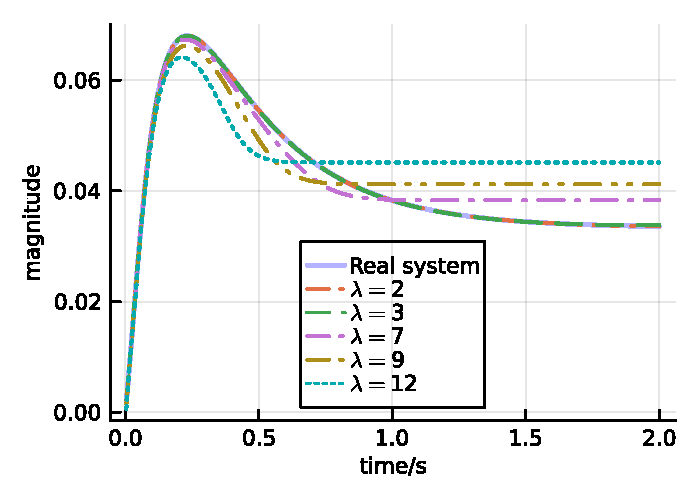
\includegraphics[scale=0.8]{figures/03_Kernel_Modelling_and_Identification_of_Neuromorphic_Elements/codes/full.pdf}
    \caption{Example 1. Approximating an LTI system with a linear kernel under different norm spaces. The solid line shows the real system. The dashed lines show the approximations.}\label{fig:full}
\end{figure}
\begin{figure}[H]
    \centering
    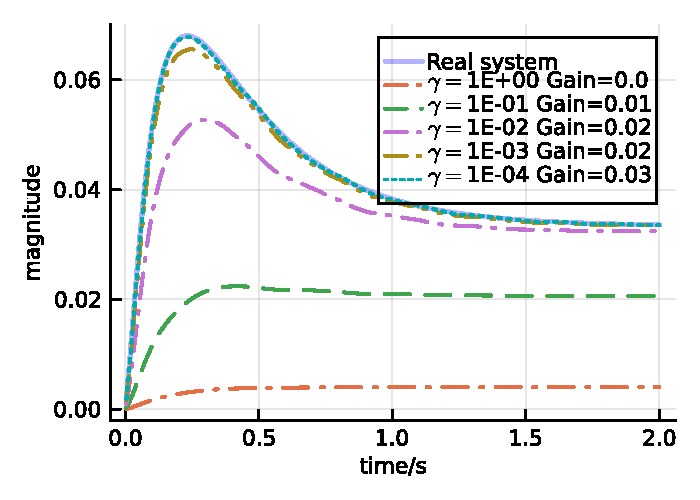
\includegraphics[scale=0.8]{figures/03_Kernel_Modelling_and_Identification_of_Neuromorphic_Elements/codes/full_reg.pdf}
    \caption{Example 1. Approximating an LTI system with a linear kernel under different regularization constants. The solid line shows the real system. The dashed lines show the approximations.}\label{fig:full_reg}
\end{figure}

As expected, stronger regularization enforces a smaller incremental $L_2$ gain in the approximated system.
\end{example}

\begin{example}[Enforcing passivity on a non-passive linear system]
In this example, we apply our framework to identify a passive linear system from data generated by the non-passive system
$$H(s)=\frac{10}{(s+1)(s+2)}.$$
For this, the scattering transform requires the modified bilinear kernel defined in Section~\ref{sec:incremental small gain_pass}.

\textcolor{examineredit}{The training data contain responses to 100 sinusoidal inputs.}

\begin{table}[H]
    \centering
    \color{examineredit}
    \small
    \renewcommand{\arraystretch}{1.15}
    \caption{\textcolor{examineredit}{Example 2. Input and sampling settings.}}
    \label{tab:kernel-example2-settings}
    \begin{tabular}{@{}p{0.22\linewidth}p{0.73\linewidth}@{}}
        \toprule
        Setting & Value or procedure \\
        \midrule
        Training inputs & \(u_{\mathrm{sin}}\) with \(A=1\), \(\omega_m=e^{-1+4(m-1)/99}\), \(m=1,\ldots,100\). \\[4pt]
        Simulation & \(0\)--\(30\)~s, with 15001 samples at intervals of \(0.002\)~s. \\[4pt]
        Input history & The latest 2001 transformed input samples, covering the final \(4\)~s. The history integral uses the trapezoidal rule. The plant is simulated from \(t=0\). \\[4pt]
        Training pairs & One pair at \(30\)~s for each response, giving 100 pairs in total. \\
        \bottomrule
    \end{tabular}
\end{table}
 We apply the scattering transform and set \(a=b=1\), \(\gamma=14.8\), and \textcolor{examineredit}{\(\lambda=1\)}. \textcolor{examineredit}{Using the weight \(w(t)=e^{\lambda t/2}\) defined on p.~\pageref{def:exponential-fading-weight}, the fading-weight constant satisfies \(c^2=\int_{-\infty}^{0}w(t)^2\,dt=\int_{-\infty}^{0}e^{\lambda t}\,dt=1/\lambda=1\). The transformed system has incremental gain bounded above by \(0.994\), so the approximated system is incrementally passive.} Figure~\ref{fig:scatter_linear} shows its Nyquist diagram.
\end{example}

\begin{figure}
    \centering
    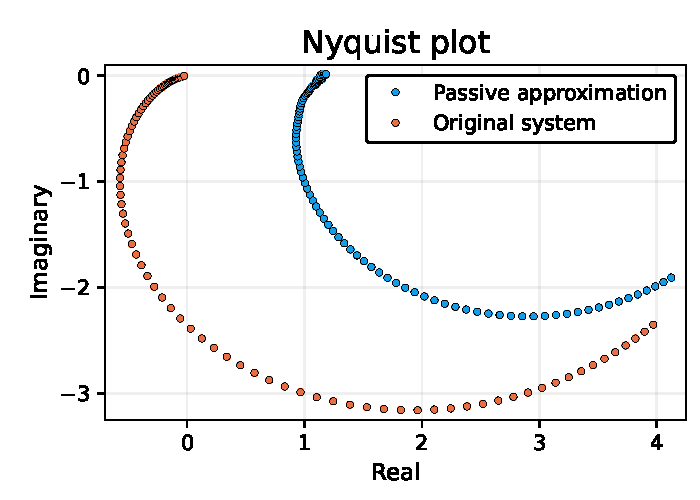
\includegraphics[scale=0.8]{figures/03_Kernel_Modelling_and_Identification_of_Neuromorphic_Elements/codes/scatter_linear_dots.pdf}
    \caption{\textcolor{examineredit}{Example 2. Approximating an LTI system from sinusoidal response data with a linear kernel and incremental passivity constraint.}}\label{fig:scatter_linear}
\end{figure}

\subsection{Nonlinear Examples}
\begin{example}[Kernel regularized learning of nonlinear systems]\label{simple nonlinear system}
We consider a saturated first-order lag with equation
\begin{IEEEeqnarray*}{rCl}
\dot{x} &=& -5x+u,\\
y&=&\operatorname{sat}(x),\\
\operatorname{sat}(x)&=&
\begin{cases}
-5 & x< -5\\
x & |x|\le5\\
5 & x> 5.
\end{cases}\\
\end{IEEEeqnarray*}
We choose an exponential fading memory with \(\lambda=4\). The model uses a Gaussian RBF kernel with \(\sigma=0.25\). \textcolor{examineredit}{We train it on sinusoidal responses and compare its step responses with those of the original system.}

\begin{table}[H]
    \centering
    \color{examineredit}
    \small
    \renewcommand{\arraystretch}{1.15}
    \caption{\textcolor{examineredit}{Example 3. Input and sampling settings.}}
    \label{tab:kernel-example3-settings}
    \begin{tabular}{@{}p{0.22\linewidth}p{0.73\linewidth}@{}}
        \toprule
        Setting & Value or procedure \\
        \midrule
        Training inputs & \(u_{\mathrm{sin}}\) with all combinations of 30 uniformly spaced frequencies in \([0,30]\)~rad/s, 50 uniformly spaced amplitudes in \([0,50]\), and \(\phi\in\{0,\pi,2\pi\}\). \\[4pt]
        Test inputs & 50 inputs \(u_{\mathrm{smooth}}\) with \(A\) uniformly spaced in \([0,50]\), \(t_0=0\), and \(\kappa=100\), over \(2\)~s. \\[4pt]
        Simulation & \(0\)--\(2\)~s, with 5000 evenly spaced samples. \\[4pt]
        Input history & All 5000 input samples, covering \(2\)~s. \\[4pt]
        Training pairs & One pair at the final sample of each response, at \(2\)~s. There are 4500 pairs in total. \\
        \bottomrule
    \end{tabular}
\end{table}

\end{example}

\begin{figure}
    \centering
    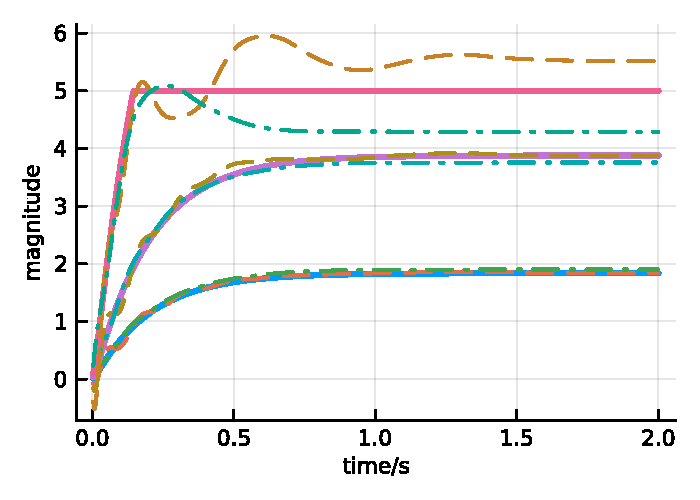
\includegraphics[scale=0.8]{figures/03_Kernel_Modelling_and_Identification_of_Neuromorphic_Elements/codes/regularisation_comb_0.0625_Nonlinear_full.pdf}
    \caption{Example 3. Solid lines are outputs of the original system. Dashed lines are outputs of an RBF kernel approximation under $\gamma=0.01$. Dash/dot lines are outputs of an RBF kernel approximation under $\gamma=1e^{-5}$.}
    \label{fig:reg1}
\end{figure}

Figure~\ref{fig:reg1} shows step responses of the original and approximate systems for two different values of the regularization constant $\gamma$. The experiments illustrate that a higher regularization constant favors a smoother input-output behaviour, consistent with the fact that regularization controls the Lipschitz constant $\beta$ and improves robustness. For $\gamma=0.01$, the Lipschitz constant of the approximated operator is about 11.

\begin{example}[Enforcing incremental passivity on a non-passive nonlinear system]
The system in Example~\ref{simple nonlinear system} is not incrementally passive \autocite{Kulkarni2001}. We construct an incrementally passive approximation as follows.

\textcolor{examineredit}{We apply the scattering transform to sinusoidal response data} and fit an incremental small-gain model with the modified RBF kernel defined in Section~\ref{sec:incremental small gain_pass}.

\begin{table}[H]
    \centering
    \color{examineredit}
    \small
    \renewcommand{\arraystretch}{1.15}
    \caption{\textcolor{examineredit}{Example 4. Input and sampling settings.}}
    \label{tab:kernel-example4-settings}
    \begin{tabular}{@{}p{0.22\linewidth}p{0.73\linewidth}@{}}
        \toprule
        Setting & Value or procedure \\
        \midrule
        Training inputs & \(u_{\mathrm{sin}}\) with \(A=15m\), \(m=1,\ldots,10\), and \(\omega=10\)~rad/s. \\[4pt]
        Test input & The training input \(u_{\mathrm{sin}}\) with \(A=150\), shown in Figure~\ref{fig:recovered_operator}. \\[4pt]
        Simulation & \(0\)--\(2\)~s, with 1000 evenly spaced samples, including both endpoints. \\[4pt]
        Input history & The latest 1000 input samples, covering \(2\)~s. \\[4pt]
        Training pairs & At sample numbers \(10,20,\ldots,1000\). This gives 100 pairs per response and 1000 pairs after scattering. \\
        \bottomrule
    \end{tabular}
\end{table}


In this case, we set $\sigma=1$, $a=b=0.1$, $\gamma=0.0005625$ and \textcolor{examineredit}{$\lambda=20$}. \textcolor{examineredit}{Using the exponential weight defined on p.~\pageref{def:exponential-fading-weight}, we have \(w(t)=e^{\lambda t/2}=e^{10t}\) and \(c^2=1/\lambda=0.05\), without additional normalization.} We scale both our input and output data after the scattering transform by $0.0005$. This scaling is used by \autocite{van_waarde_kernel-based_2023} so that the algorithm gives a less conservative bound. \textcolor{examineredit}{With \(s=0.0005\), the approximation in the original coordinates is \(\widehat E(u')=s^{-1}\widehat E_s(su')\), where \(\widehat E_s\) is fitted to the scaled data.}
\textcolor{examineredit}{With these settings, the trained model satisfies \(\beta^2(b+ac^2)<0.998<1\) and therefore has incremental small gain.}

Finally, we use one of the training trajectories to test whether the incrementally passive approximation can be recovered through the scattering transform, by placing the trained operator in the feedback loop shown in Figure~\ref{fig:scattering}. The result is shown in Figure~\ref{fig:recovered_operator}.

\begin{figure}
    \centering
    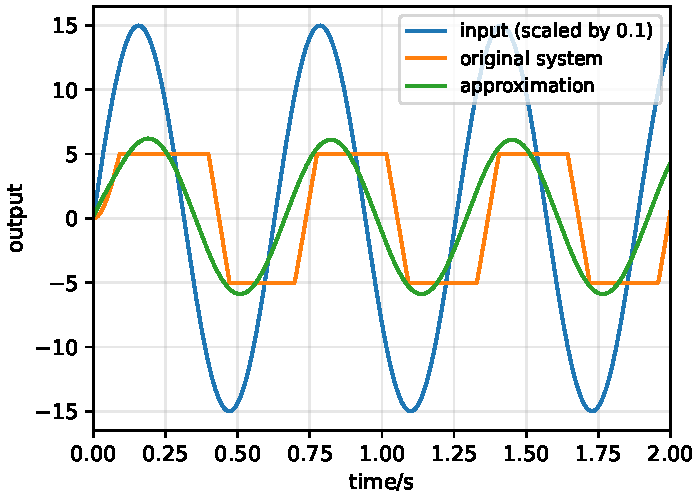
\includegraphics[scale=0.8]{figures/03_Kernel_Modelling_and_Identification_of_Neuromorphic_Elements/codes/scatter_simple.pdf}
    \caption{\textcolor{examineredit}{Example 4. Approximating a nonlinear system with an RBF kernel and incremental passivity constraint. Response to a sine wave with angular frequency \(10\)~rad/s and amplitude 150.}}\label{fig:recovered_operator}
\end{figure}

We can see that the output of the incrementally passive approximation is similar to the output of the linear part in the original nonlinear system, with a small phase shift.

\end{example}

\subsection{Kernel Learning of Nonlinear Systems with Gain Scheduling Kernel}

The gain-scheduling kernel encodes memristive and time-scale-separation properties in the learned system. This subsection applies the gain-scheduling kernel (GS kernel) to two examples: the simple nonlinear system in the previous subsection and the ion-channel currents of a spiking neuron, viewed as currents produced by memristive elements. With two distinct time-scales in the kernel model, the approximations generalize from only a few step responses.

\textcolor{examineredit}{To compare generalization, we train an RBF model and a GS model on step and sinusoidal responses of the nonlinear system below.}
\begingroup
\color{examineredit}
\[
\begin{aligned}
\dot{x} &= -5x+u,\\
y &= \operatorname{sat}(x),\\
\operatorname{sat}(x) &=
\begin{cases}
-0.5 & x<-0.5,\\
x & |x|\leq0.5,\\
0.5 & x>0.5.
\end{cases}
\end{aligned}
\]
\endgroup
\textcolor{examineredit}{Here the saturation limits are \(\pm0.5\), whereas the preceding nonlinear examples use \(\pm5\).}

\textcolor{examineredit}{We first train both models on the step-response data set and test them on a sinusoidal input. We then train them on the sinusoidal data set and test them on a step input.}

\begin{table}[H]
    \centering
    \color{examineredit}
    \small
    \renewcommand{\arraystretch}{1.15}
    \caption{\textcolor{examineredit}{GS comparison. Input and sampling settings for both training sets.}}
    \label{tab:kernel-gs-settings}
    \begin{tabular}{@{}p{0.22\linewidth}p{0.73\linewidth}@{}}
        \toprule
        Setting & Value or procedure \\
        \midrule
        Step training set & 20 inputs \(u_{\mathrm{step}}\) with \(A=-9,-8,\ldots,10\) and \(t_0=0\). Test on \(u_{\mathrm{sin}}\) with \(A=9\), \(\omega=10\)~rad/s. \\[4pt]
        Sinusoidal training set & 20 inputs \(u_{\mathrm{sin}}\) with \(A=1,\ldots,10\) and \(\omega\in\{5,10\}\)~rad/s. Test on \(u_{\mathrm{step}}\) with \(A=8\), \(t_0=0\). \\[4pt]
        Simulation & \(0\)--\(4\)~s, with 1000 evenly spaced samples per response. \\[4pt]
        Input history & The latest 1000 input samples, covering \(4\)~s. \\[4pt]
        Training pairs & At sample numbers \(20,40,\ldots,1000\). This gives 50 pairs per response and 1000 pairs in each training set. \\
        \bottomrule
    \end{tabular}
\end{table}


The results are shown in Figures~\ref{fig:StSinRBF}--\ref{fig:SinStGSK}. As before, $\lambda$ refers to the decay rate of the fading-memory weight $w$.
\begin{figure}[H]
    \centering
    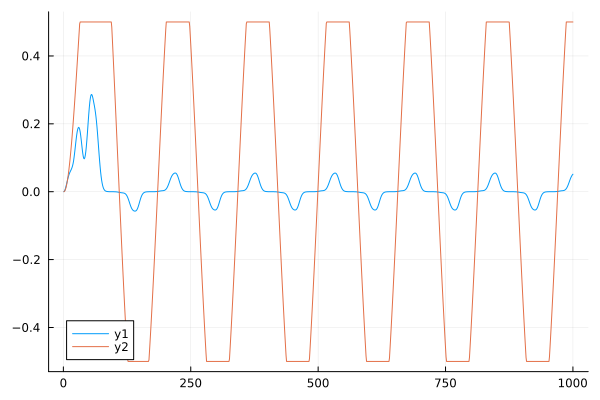
\includegraphics[scale=0.6]{figures/03_Kernel_Modelling_and_Identification_of_Neuromorphic_Elements/codes/stepTrainSinTest_RBF.png}
    \caption{RBF model trained with step responses and tested on a sine wave. The orange line is the true response. The blue line is the response from the approximated system $\gamma=0.0006$, $\sigma=1$, $\lambda=5$.}
    \label{fig:StSinRBF}
\end{figure}
\begin{figure}[H]
    \centering
    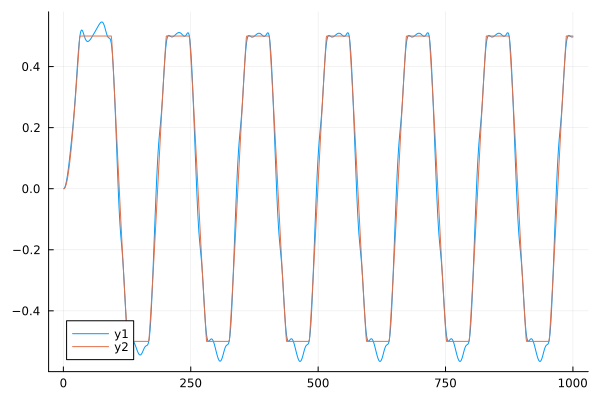
\includegraphics[scale=0.6]{figures/03_Kernel_Modelling_and_Identification_of_Neuromorphic_Elements/codes/stepTrainSinTest_GSK.png}
    \caption{GS model trained with step responses and tested on a sine wave. The orange line is the true response. The blue line is the response from the approximated system $\gamma=0.0006$, $\sigma=1$, $\lambda=5$.}
    \label{fig:StSinGSK}
\end{figure}
\begin{figure}[H]
    \centering
    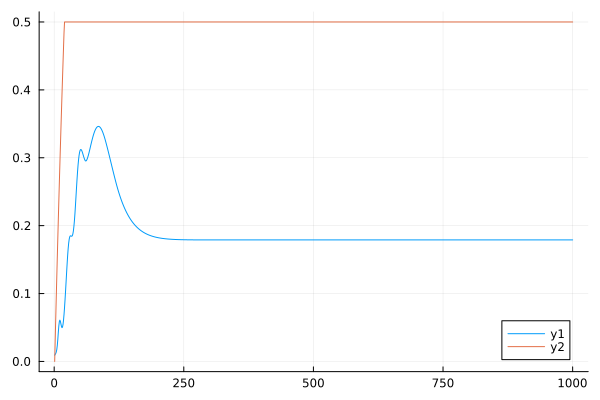
\includegraphics[scale=0.6]{figures/03_Kernel_Modelling_and_Identification_of_Neuromorphic_Elements/codes/sinTrainStepTest_RBF.png}
    \caption{RBF model trained with sine responses and tested on a step input. The orange line is the true response. The blue line is the response from the approximated system $\gamma=0.0006$, $\sigma=1$, $\lambda=5$.}
    \label{fig:SinStRBF}
\end{figure}
\begin{figure}[H]
    \centering
    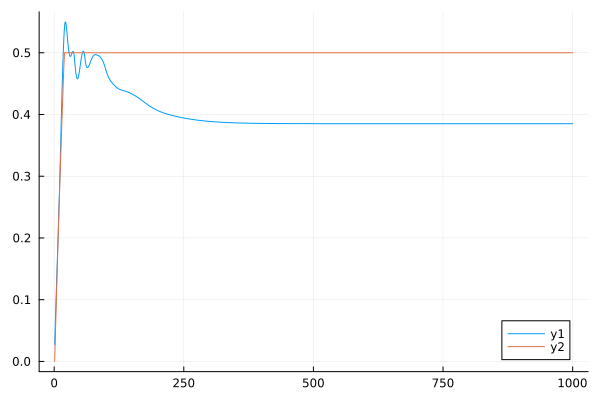
\includegraphics[scale=0.6]{figures/03_Kernel_Modelling_and_Identification_of_Neuromorphic_Elements/codes/sinTrainStepTest_GSK.png}
    \caption{GS model trained with sine responses and tested on a step input. The orange line is the true response. The blue line is the response from the approximated system $\gamma=0.0006$, $\sigma=1$, $\lambda=5$.}
    \label{fig:SinStGSK}
\end{figure}
Figures~\ref{fig:StSinRBF} and~\ref{fig:SinStRBF} show the RBF results, while Figures~\ref{fig:StSinGSK} and~\ref{fig:SinStGSK} show the corresponding GS-kernel results. In both train-test directions, the GS kernel generalises better than the RBF kernel.

Next, we use the GS model to approximate the sodium and potassium conductance currents of the HH model from a small set of step and impulse responses. This tests whether encoding memristive structure in the kernel improves data efficiency.

The potassium channel has the form 
\begin{eqnarray}
y=36n^4(u-V_K)\\
\dot{n} = \alpha_n(u)(1-n)-\beta_n(u)n,\\
\alpha_n(u) = \frac{0.1 - 0.01(-V_r+u)}{exp(1 - 0.1(-V_r+u))- 1}\\
\beta_n(u) = \frac{0.125}{exp(0.0125(-V_r+u))}\\
\end{eqnarray}
with $V_r= -65.1$ and $V_K  = -77$. $V_r$ is the resting potential of the neuron. 

\textcolor{examineredit}{We identify the potassium-channel model from voltage-step responses.} The potassium-channel result is shown in Figure~\ref{fig:IonChannelKOpenLoop}.

\begin{table}[H]
    \centering
    \color{examineredit}
    \small
    \renewcommand{\arraystretch}{1.15}
    \caption{\textcolor{examineredit}{Potassium channel. Input and sampling settings.}}
    \label{tab:kernel-potassium-settings}
    \begin{tabular}{@{}p{0.22\linewidth}p{0.73\linewidth}@{}}
        \toprule
        Setting & Value or procedure \\
        \midrule
        Training inputs & 50 voltage inputs \(u_{\mathrm{smooth}}\) with \(B=-65.1\)~mV, final voltages \(B+A=28,26,\ldots,-70\)~mV, \(t_0=10\)~s, and \(\kappa=1000\). \\[4pt]
        Initial gate state & \(n(0)=n_\infty(-65.1)\). \\[4pt]
        Simulation & \(0\)--\(20\)~s, with 2000 evenly spaced samples. \\[4pt]
        Input history & The latest 1000 input samples, covering about \(10\)~s. \\[4pt]
        Training pairs & At sample numbers \(1050,1100,\ldots,2000\). This gives 20 pairs per response and 1000 pairs in total. \\
        \bottomrule
    \end{tabular}
\end{table}


\begin{figure}[H]
    \centering
    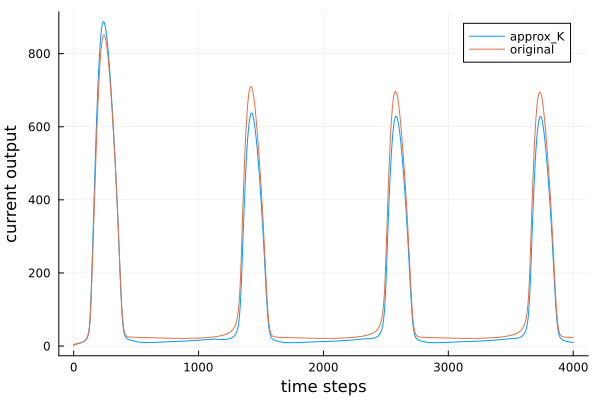
\includegraphics[scale=0.6]{figures/03_Kernel_Modelling_and_Identification_of_Neuromorphic_Elements/codes/ion_channel_K_open_loop.png}
    \caption{Open-loop response of the GS model of the potassium channel compared with the true potassium channel. The orange line is the true response and the blue line is the response from the approximated system $\gamma=0.0001$, $\sigma=10$, $\lambda=0.2$.}
    \label{fig:IonChannelKOpenLoop}
\end{figure}

The sodium channel has a form 
\begin{eqnarray}
y=120*m^3*h*(u-V_Na)\\
\dot{m}=\alpha_m(u)(1-m)-\beta_m(u)*m\\
\dot{h}=\alpha_h(u)(1-h)-\beta_h(u)*h\\
\alpha_m(u) = \frac{2.5 - 0.1*(-V_r+u)}{exp(2.5 - 0.1*(-V_r+u))- 1}\\
\beta_m(u) = \frac{4}{exp((-V_r+u)/18)}\\
\alpha_h(u) = \frac{0.07}{exp(0.05*(-V_r+u))}\\
\beta_h(u) = \frac{1}{exp(3 - 0.1*(-V_r+u))+ 1}\\
\end{eqnarray}
with $V_r= -65.1$ and $ V_Na= 50$. 

The sodium channel is more complex than the potassium channel because it combines two nonlinear gating subsystems. Since these subsystems operate on different time scales \cite{hodgkin_quantitative_1952}, we use two kernel constructions: one gain-scheduling kernel for the potassium channel with one time scale, and one gain-scheduling kernel for the sodium channel with two time scales.

\begin{definition}{Gain-scheduling kernel for fading memory system (Type 2)}
\begin{eqnarray}
  k(u,v)=exp\left(\frac{-(\langle u,w\rangle-\langle v,w\rangle)^2}{2\sigma^2}\right)\langle u,v\rangle_{w}(u(0)-V_{a})(v(0)-V_{a}) 
\end{eqnarray}
\end{definition}

\begin{definition}{Gain-scheduling kernel for fading memory system (Type 3)}
\begin{equation}
\begin{aligned}
  \textcolor{examineredit}{k(u,v)} &\textcolor{examineredit}{=\exp\left(\frac{-(\langle u,w\rangle-\langle v,w\rangle)^2}{2\sigma_1^2}\right)}\\
  &\textcolor{examineredit}{\quad{}\times\exp\left(\frac{-(\langle u,w_2\rangle-\langle v,w_2\rangle)^2}{2\sigma_2^2}\right)}\\
  &\textcolor{examineredit}{\quad{}\times\langle u,v\rangle_{w}(u(0)-V_{a})(v(0)-V_{a}).}
\end{aligned}
\end{equation}
\end{definition}

Here \(V_a\) is the reversal voltage of the channel: \(V_a=V_K=-77\)~mV for potassium and \(V_a=V_{Na}=50\)~mV for sodium. This is a product of three kernels, so it remains a kernel \cite{paulsen_introduction_2016}. The two decaying weights \(w\) and \(w_2\) represent the two channel time scales. This kernel is not \emph{non-expansive}.

\textcolor{examineredit}{We identify the sodium-channel model from voltage-pulse responses at different bias voltages.} Figure~\ref{fig:IonChannelNaOpenLoop} shows the result. Here \(\lambda_w\) and \(\lambda_{w_2}\) are the decay rates of \(w\) and \(w_2\).

\begin{table}[H]
    \centering
    \color{examineredit}
    \small
    \renewcommand{\arraystretch}{1.15}
    \caption{\textcolor{examineredit}{Sodium channel. Input and sampling settings.}}
    \label{tab:kernel-sodium-settings}
    \begin{tabular}{@{}p{0.22\linewidth}p{0.73\linewidth}@{}}
        \toprule
        Setting & Value or procedure \\
        \midrule
        Training inputs & 40 voltage inputs \(u_{\mathrm{pulse}}\) with \(B=20,17.5,\ldots,-77.5\)~mV, \(A=1000\), \(t_{\mathrm{on}}=13\)~s, \(t_{\mathrm{off}}=13.01\)~s, and \(\kappa=100\). \\[4pt]
        Initial gate states & \(m(0)=m_\infty(-65.1)\), \(h(0)=h_\infty(-65.1)\). \\[4pt]
        Simulation & \(0\)--\(15\)~s, with 1500 evenly spaced samples. \\[4pt]
        Input history & The latest 1500 input samples, covering \(15\)~s. \\[4pt]
        Training pairs & Use both sample lists \(60,120,\ldots,1500\) and \(1308,1316,\ldots,1500\). Repeated sample numbers give separate pairs. There are 50 pairs per response and 2000 pairs in total. \\
        \bottomrule
    \end{tabular}
\end{table}


\begin{figure}[H]
    \centering
    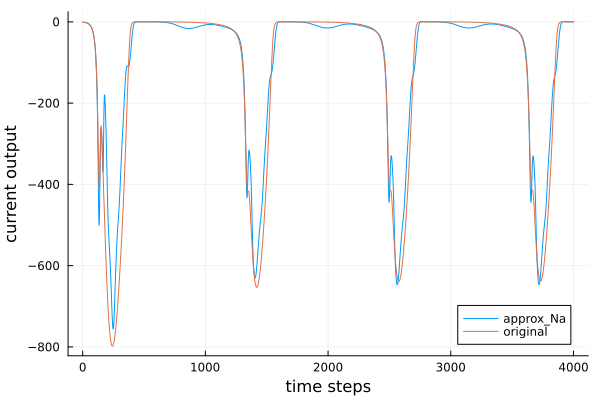
\includegraphics[scale=0.5]{figures/03_Kernel_Modelling_and_Identification_of_Neuromorphic_Elements/codes/ion_channel_Na_open_loop.png}
    \caption{Open-loop response of the GS model of the sodium channel compared with the true sodium channel. The orange line is the true response and the blue line is the response from the approximated system \(\gamma=10^{-7}\), \(\sigma_1=9.5\), \(\sigma_2=2.5\), \(\lambda_w=0.2\), and \(\lambda_{w_2}=1.5\).}
    \label{fig:IonChannelNaOpenLoop}
\end{figure}

\textcolor{examineredit}{Both channel models are first tested with a membrane-voltage trace generated by the full HH model under constant injected current.}

Both approximations predict the spike-input responses reasonably well. We next test closed-loop performance by replacing the sodium and potassium conductance-current models in the HH model with their approximations. The closed-loop response and the corresponding input are shown in Figures~\ref{fig:HHClosedLoop} and~\ref{fig:HHClosedLoopInput}.

\begingroup
\color{examineredit}
The closed-loop HH input is a smoothed random current,
\[
I_i=3+\frac{1}{100}\sum_{r=i}^{i+500}\xi_r,\qquad
\xi_1,\ldots,\xi_{4500}\ \overset{\mathrm{iid}}{\sim}\mathcal U[-50,50].
\]
This uses a 501-term sum divided by 100. The random seed was not recorded. To reproduce the figures, use the saved 4000-sample vector in \path{Kernel_work/code/test2_input.txt}, rather than drawing a new input.
\endgroup

\begin{table}[H]
    \centering
    \color{examineredit}
    \small
    \renewcommand{\arraystretch}{1.15}
    \caption{\textcolor{examineredit}{HH parameters, initial conditions, and test settings.}}
    \label{tab:kernel-hh-settings}
    \begin{tabular}{@{}p{0.22\linewidth}p{0.73\linewidth}@{}}
        \toprule
        Setting & Value or procedure \\
        \midrule
        Membrane and leak & \(C_m=1\), \(\bar g_L=0.3\), \(E_L=-54.387\) in \eqref{eq:HH_voltage_recalled}. \\[4pt]
        Ion channels & \(\bar g_K=36\), \(\bar g_{Na}=120\), \(E_K=-77\), \(E_{Na}=50\). \\[4pt]
        Initial conditions & The full HH model starts at \(V(0)=-65.1\), with its gates at their steady-state values at this voltage. For the learned sodium and potassium models, all voltage samples in the initial input histories are set to \(-65.1\)~mV. \\[4pt]
        Open-loop test & Constant injected current \(20\) model units over \(40\)~s. Forward Euler with step \(0.01\)~s. \\[4pt]
        Closed-loop test & 3999 forward-Euler updates of length \(0.01\), using current samples \(1,\ldots,3999\). The 4000 stored voltage and current samples are plotted on an evenly spaced \(0\)--\(40\) time axis. \\
        \bottomrule
    \end{tabular}
\end{table}

\begin{figure}[H]
    \centering
    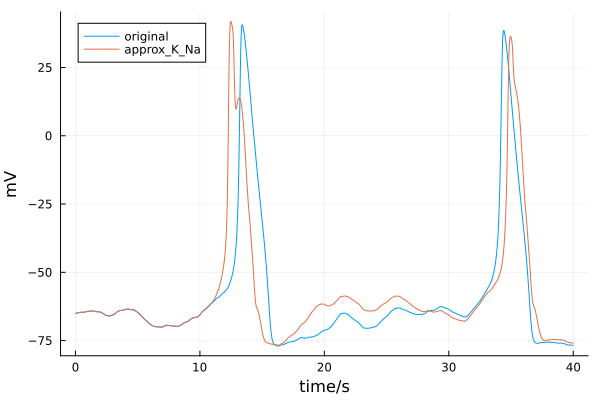
\includegraphics[scale=0.6]{figures/03_Kernel_Modelling_and_Identification_of_Neuromorphic_Elements/codes/HH_model_test2_summary.png}
    \caption{Closed-loop response of the approximated model. Blue line is the true response and Orange line is the response from the approximated system.}
    \label{fig:HHClosedLoop}
\end{figure}

\begin{figure}[H]
    \centering
    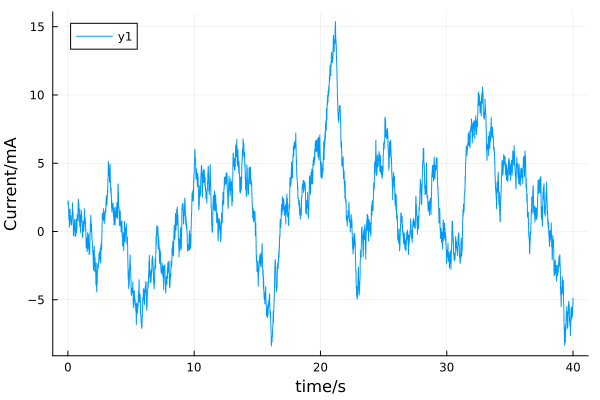
\includegraphics[scale=0.6]{figures/03_Kernel_Modelling_and_Identification_of_Neuromorphic_Elements/codes/HH_model_test2_summary_input.png}
    \caption{Current input}
    \label{fig:HHClosedLoopInput}
\end{figure}
Figure~\ref{fig:HHClosedLoop} compares the approximated and true responses. The approximated model captures spike timing well, although the spike shapes differ. Figure~\ref{fig:HHClosedLoopInput} shows the current input used for the test. The result indicates that the model captures the dominant conductance structure from limited data.


\section{Conclusion}\label{sec:conclusions}

This chapter addressed the \emph{element-level} bottleneck of the dissertation: how to
identify a neuromorphic element and, in particular, its conductances, from
data in a representation that preserves the memristive structure and time-scale separation
needed for event-based networks. Building on the fading-memory abstraction introduced in
Chapter~\ref{chap:conductance-memristive-fm}, we adopted the operator-theoretic view that
any time-invariant causal system can be represented by a \emph{memory functional} mapping
past inputs to the current output. The key engineering move is therefore to learn this
memory functional directly in an RKHS, rather than learning an implicit state-space model
whose internal coordinates may be difficult to identify, simulate, or preserve under
interconnection.

The RKHS formulation yields a practical modelling methodology for memristive conductance elements:
(i) \emph{fit from input-output data} using kernel ridge regression and the representer theorem,
(ii) \emph{regularize incremental input-output properties} that remain meaningful under feedback and network interconnection, and
(iii) \emph{encode physical structure} through kernel design, in particular memristive behaviour and time-scale separation.

In a large neuromorphic network, the learned elements must fit the data and remain well behaved under interconnection, modelling error, and perturbation. By working with
kernels with finite Lipschitz constants, the learned element can be constrained
to satisfy incremental small-gain properties. Through scattering-type transformations, the
same viewpoint can be extended to other incremental constraints, including incremental
passivity. Through encoding the time-scale separation and memristive structure into the kernel, the learned model can be made more data-efficient and better aligned with the physical interpretation of conductance-based dynamics.

The gain-scheduling kernels encode memristive structure and time-scale separation. They show
how memristive behaviour and time-scale separation can be built directly into the
kernel, improving generalization when data are sparse or restricted to a limited
set of stimuli. The resulting learned model is data-consistent and aligned with the physical interpretation of conductance-based dynamics.

This chapter studies incremental passivity for learned memristive conductance elements. When isolated from regenerative feedback, ionic conductances have a passive dissipative role in the circuit. The regularizer biases the learned current toward this behaviour, consistent with viewpoints based on monotonicity and incremental dissipativity \cite{sepulchre_spiking_2022,sepulchre_incremental_2022}.


The proposed abstraction for an ion-channel conductance is a causal fading-memory functional. Its kernel encodes memristive structure and time-scale separation, and regularization constrains its incremental input-output behaviour. The next chapter introduces rebound excitability and its use in network motifs.
